\documentclass[10pt]{beamer}

\usetheme{metropolis}
\usepackage{appendixnumberbeamer}
\usepackage[utf8]{inputenc}
\usepackage[russian,francais]{babel}
\usepackage{booktabs}
\usepackage[scale=2]{ccicons/ccicons}
\usepackage{pifont}
\usepackage{pgfplots}
\usepgfplotslibrary{dateplot}

\usepackage{xspace}
\newcommand{\themename}{\textbf{\textsc{metropolis}}\xspace}
%%\usepackage{polyglossia}
%%    \setdefaultlanguage{french} % main language
%%    \setotherlanguages{russian, hindi, greek, hebrew} % other languages 
%%\graphicspath{{images/}}	% Put all images in this directory. Avoids clutter.
%%\setmainfont{Latin Modern Roman}
%%\setsansfont{Latin Modern Sans}
%%\setmonofont{Latin Modern Mono}
%%\setmainfont[Ligatures=TeX]{Times New Roman}
%%\newfontfamily{\cyrillicfonttt}{Times New Roman}[Script=Cyrillic]

\usetheme{metropolis}
\usepackage{appendixnumberbeamer}
\usepackage[utf8]{inputenc}
\usepackage[russian,francais]{babel}
\usepackage{booktabs}
\usepackage[scale=2]{ccicons}
%\usepackage{xcolor}
\usepackage{wrapfig}
\usepackage{subcaption}
\usepackage{pgfplots}
\usepgfplotslibrary{dateplot}
\usepackage{graphicx}
\usepackage{xspace}
\usepackage{hyperref}
\usepackage{arydshln}
\usepackage{pifont}
\usepackage{enumitem}
\usepackage{xcolor}
\usepackage{amsmath}
%\usepackage{minted}
%%\usepackage{polyglossia}
%%    \setdefaultlanguage{french} % main language
%%    \setotherlanguages{russian, hindi, greek, hebrew} % other languages 
%%\graphicspath{{images/}}	% Put all images in this directory. Avoids clutter.
%%\setmainfont{Latin Modern Roman}
%%\setsansfont{Latin Modern Sans}
%%\setmonofont{Latin Modern Mono}
%%\setmainfont[Ligatures=TeX]{Times New Roman}
%%\newfontfamily{\cyrillicfonttt}{Times New Roman}[Script=Cyrillic]









\definecolor{greenperso}{RGB}{68,117,104}
\definecolor{greenblue}{RGB}{95,179,176}



\title{Programmation de Modèles Linguistiques 2, \\ L6SOPRG L3}
%\subtitle{Crédits : %\& Angélique Allaire, ObTIC}
%\subtitle{A modern beamer theme}
\date{}
\author{Caroline Koudoro-Parfait\\ \quad {caroline.parfait@sorbonne-universite.fr\\}}
\institute{Observatoire des Textes des Idées et des Corpus - Obtic,\\ Sorbonne Center for Artificial Intelligence - SCAI,\\ Sens Textes Informatiques Histoire - STIH EA 4509, Sorbonne Université}
 \titlegraphic{\hfill
\includegraphics[height=.7cm]{images/sorbonne.png}}
\begin{document}
\maketitle

%\begin{frame}{Plan de la présentation}
%  \setbeamertemplate{section in toc}[sections numbered]
%  \tableofcontents[hideallsubsections]
%\end{frame}
\begin{frame}
  \frametitle{Plan du cours}
\tableofcontents

\end{frame}


\section{Github : qu'est-ce que c'est et à quoi ça sert ?}
\begin{frame}
  \frametitle{C'est quoi Github ?}
\begin{itemize}
\item \ding{81} service web de dépôt et de versionnage de code
\item \ding{81} s'appuie sur logiciel de gestion de versions Git\footnote{\url{https://git-scm.com/}}
\item \ding{81} développé avec Ruby on Rails et Erlang
\item \ding{81} propose des comptes professionnels payants
\item \ding{81} des comptes gratuits pour les projets de logiciels libres

\end{itemize}

\end{frame}


\begin{frame}
  \frametitle{A quoi ça sert ?}
\begin{itemize}
\item \ding{81} hébergement développement de logiciels
\item \ding{81} gestion de développement de logiciels
\item \ding{81} dépôt public de projets libres \& dépôt privé d'entreprises
\item \ding{81} Travaille collaboratif sur un même programme
\end{itemize}
\end{frame}

\section{Github : fonctionnalités et usages}
\begin{frame}
  \frametitle{Les fonctionnalités}
\begin{itemize}
\item \ding{81} contrôle d'accès des collaborateurs
\item \ding{81} fonctionnalités pour la collaboration : système de branches
\item \ding{81} suivi des bugs
\item \ding{81} gestion des tâches 
\item \ding{81} Documentation du projet : un README a rédigé en Markdown\footnote{\url{https://docs.framasoft.org/fr/grav/markdown.html}}
\item \ding{81} Choisir une licence libre\footnote{\url{https://creativecommons.org/licenses/}}
\end{itemize}
\end{frame}

\begin{frame}
  \frametitle{Comment ça marche ?}

\begin{itemize}
\item \ding{81} Il existe un dépôt local (votre machine) et un dépôt distant (le serveur) 
\item \ding{81} Ils sont liés par un fichier caché : .git
\item \ding{81} Vous travaillez en local
\item \ding{81} Vous partagé sur le serveur
\item \ding{81} Vous pouvez récupérer votre travail
\item \textcolor{green}{\ding{81}} Les utilisateurs peuvent cloner vos dépôts publics
\item \ding{81} Les collègues ayant la permission sur vos dépôt publics et privés peuvent : 
\begin{itemize}
\item \textcolor{green}{\ding{52}} récupérer vos dépôts 
\item \textcolor{green}{\ding{52}} commit et push leurs modifications
\end{itemize}
\end{itemize}
\end{frame}

\begin{frame}
  \frametitle{Comment ça marche ?}
\begin{itemize}
\item \ding{80} Toujours vérifier le statut du dépôt == à jour local + serveur ?
\item \textcolor{orange}{\ding{42}} git pull == mise à jour (maj) dépôt local
\item \ding{80} partager sur le serveur
\begin{itemize}
\item \textcolor{orange}{\ding{42}} git commit "décrire la maj" == lancer le partage sur le serveur
\item \textcolor{orange}{\ding{42}} git push == déposer sur le serveur
\end{itemize}
\end{itemize}
\end{frame}

\section{Github desktop : description de l'interface et usage}
\begin{frame}
  \frametitle{créer un compte sur github}

Rendez-vous sur la page : 
\begin{figure}
\caption{\url{https://github.com/.}}
  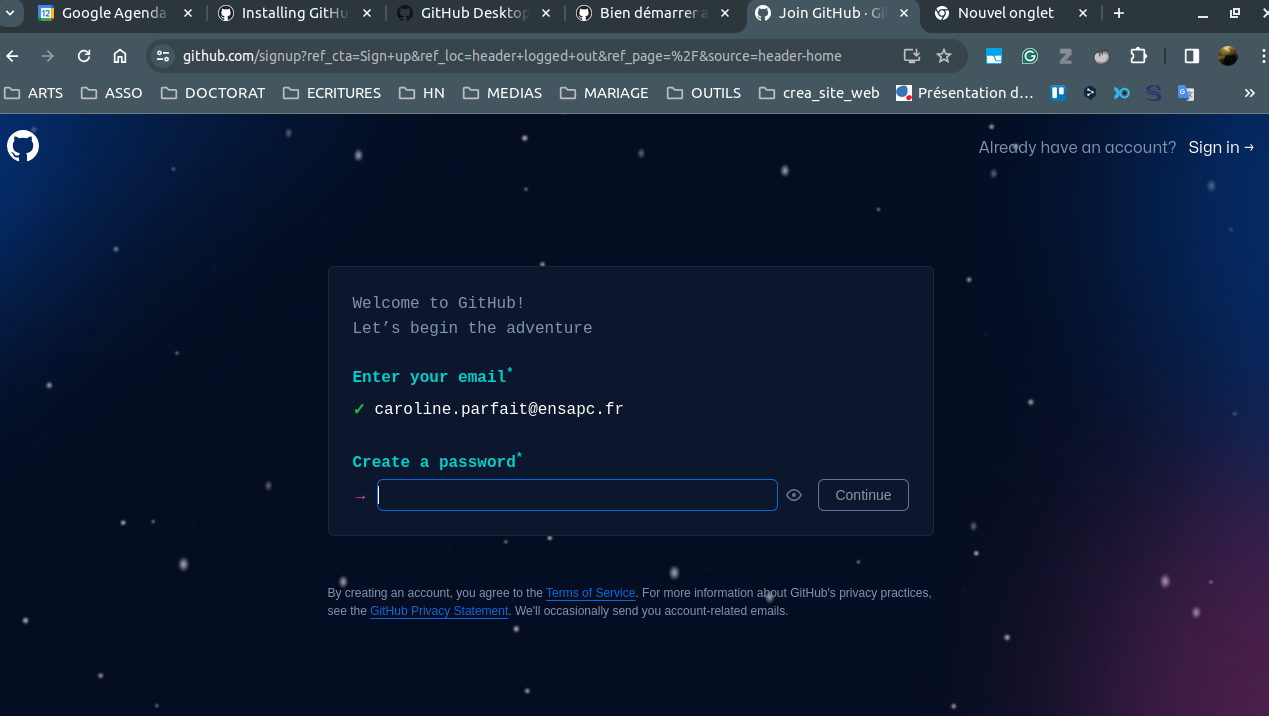
\includegraphics[width=6cm]{images/github_inscription.png}
  
  \end{figure}
  
\end{frame}

\begin{frame}
  \frametitle{télécharger github desktop}

Rendez-vous sur la page : 
\begin{figure}
\caption{\url{https://desktop.github.com/?ref_cta=download+desktop&ref_loc=installing+github+desktop&ref_page=docs}}
  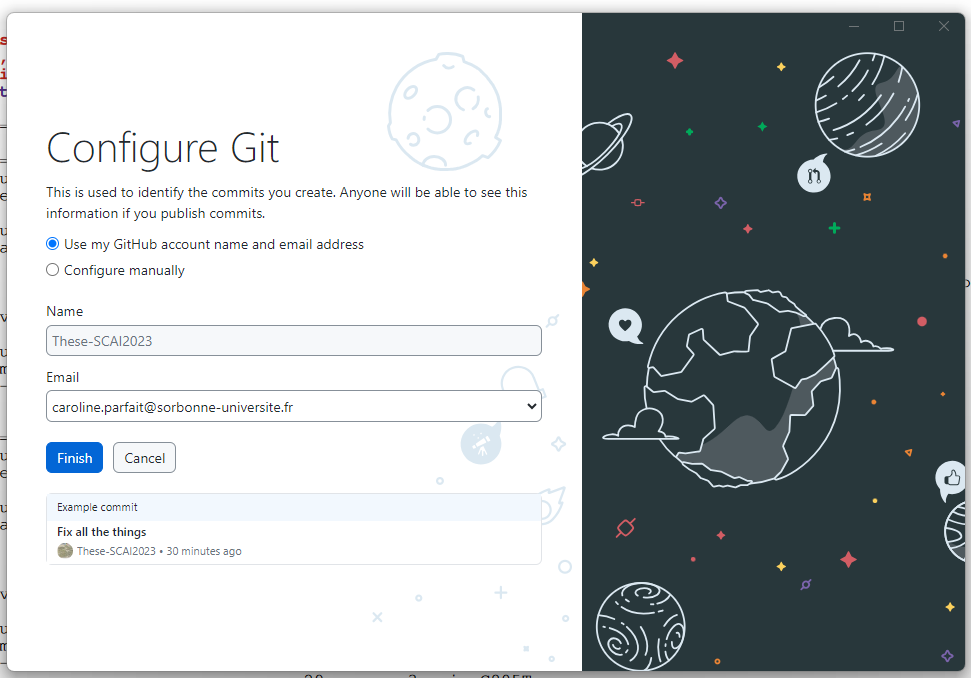
\includegraphics[width=6cm]{images/github_desktop_connect.png}
  
  \end{figure}

\ding{52} L'interface Desktop est liée à votre compte Github  
  
\end{frame}

\begin{frame}
  \frametitle{Cloner un dépôt existant ...}

Rendez-vous sur la page : 
\begin{figure}
\caption{\url{https://docs.github.com/en/desktop/adding-and-cloning-repositories/cloning-a-repository-from-github-to-github-desktop}}
  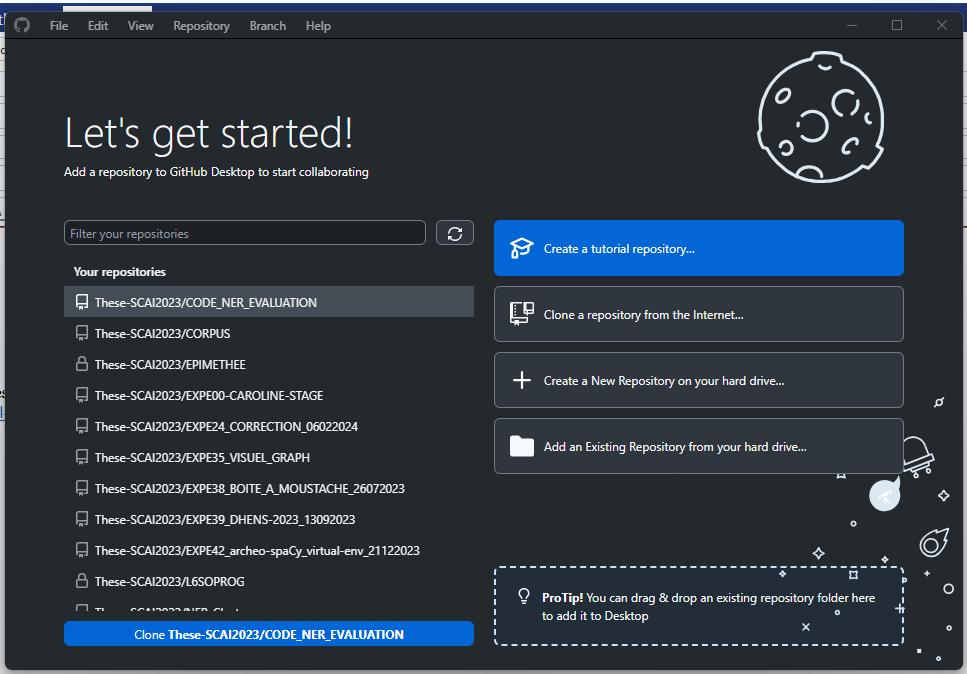
\includegraphics[width=6cm]{images/github_desktop_connect2.png}
  \end{figure}
  
\end{frame}

\begin{frame}
  \frametitle{Cloner un dépôt existant ...}

Rendez-vous sur la page : 
\begin{figure}
\caption{\url{https://docs.github.com/en/desktop/adding-and-cloning-repositories/cloning-a-repository-from-github-to-github-desktop}}
  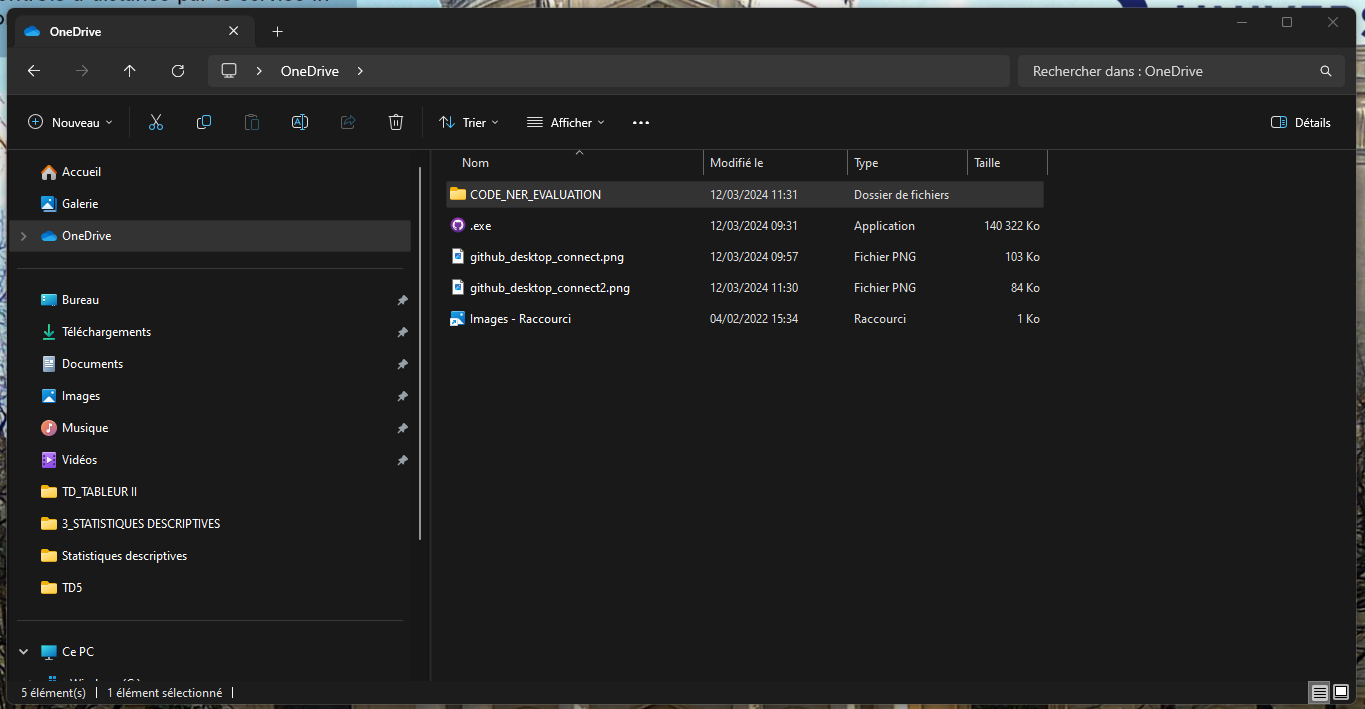
\includegraphics[width=6cm]{images/github_desktop_connect3.png}
  \end{figure}
 \ding{52} ... le dépôt est en local, sur votre machine 
\end{frame}

\begin{frame}
  \frametitle{Nouvelle version du programme cloné : commit}

Rendez-vous sur la page : 
\begin{figure}
\caption{https://docs.github.com/en/desktop/making-changes-in-a-branch/committing-and-reviewing-changes-to-your-project-in-github-desktop}
  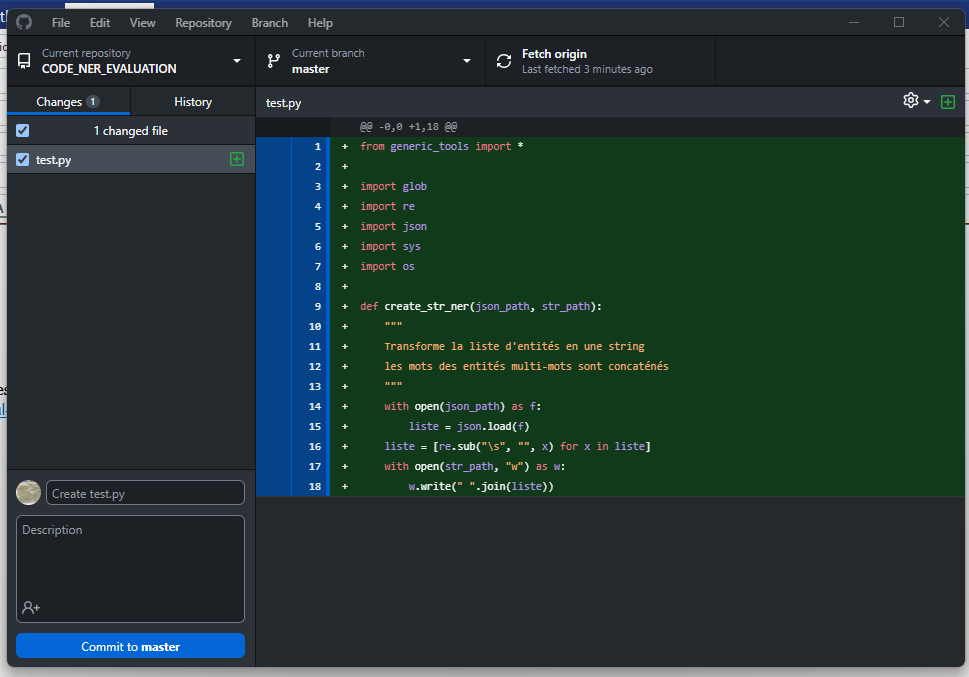
\includegraphics[width=6cm]{images/github_desktop_connect4.png}
  \end{figure}

\end{frame}



\begin{frame}
  \frametitle{Nouvelle version du programme cloné : push}

Rendez-vous sur la page : 
\begin{figure}
\caption{\url{https://docs.github.com/en/desktop/making-changes-in-a-branch/pushing-changes-to-github-from-github-desktop}}
  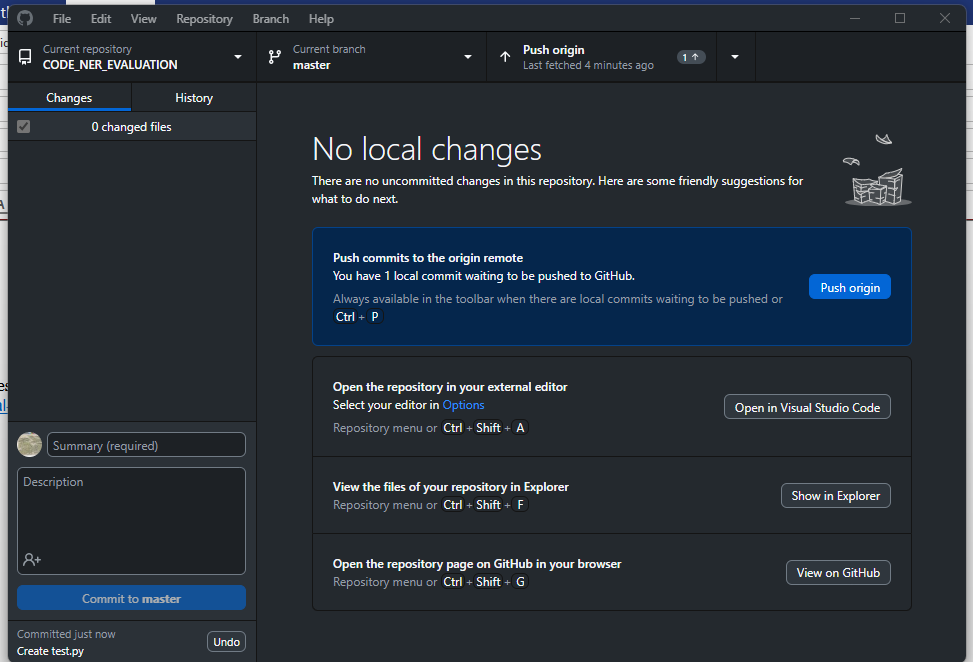
\includegraphics[width=6cm]{images/github_desktop_connect5.png}
  \end{figure}
  
\end{frame}

\begin{frame}
  \frametitle{... push du dépôt sur le serveur}

Rendez-vous sur la page : 
\begin{figure}
\caption{\url{https://docs.github.com/en/desktop/making-changes-in-a-branch/pushing-changes-to-github-from-github-desktop}}
  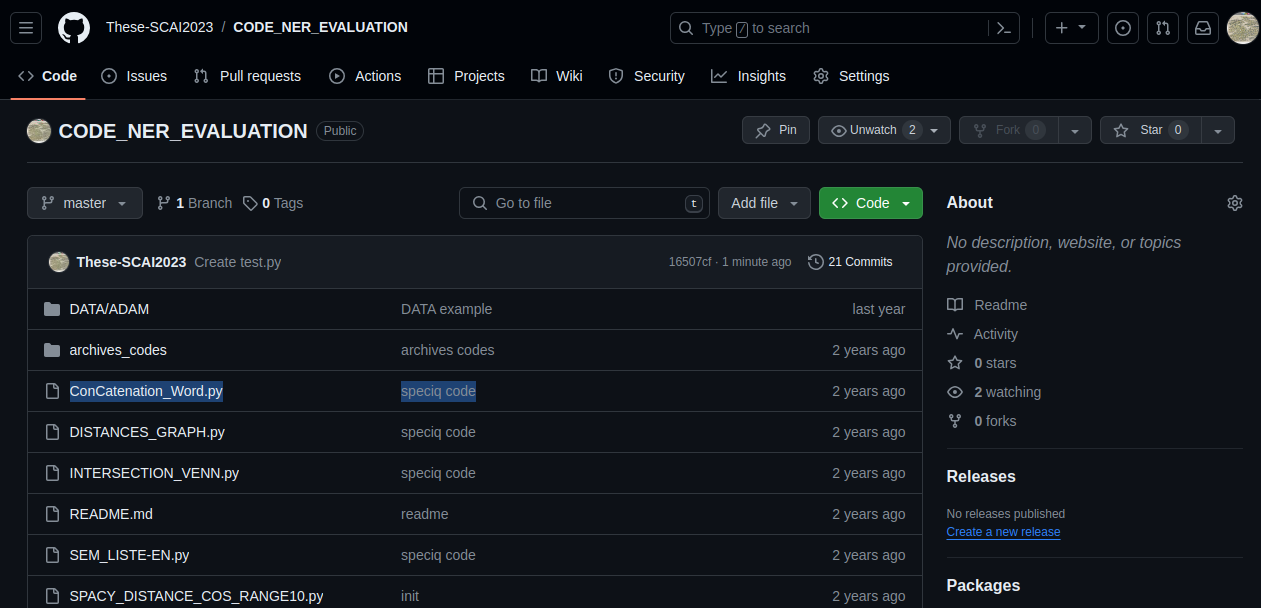
\includegraphics[width=6cm]{images/github_push_compte.png}
  \end{figure}
  
\end{frame}

\begin{frame}
  \frametitle{Récupérer le travail des collègues : pull request}

Rendez-vous sur la page : 
\begin{figure}
\caption{\url{https://docs.github.com/en/desktop/working-with-your-remote-repository-on-github-or-github-enterprise/viewing-a-pull-request-in-github-desktop}}
  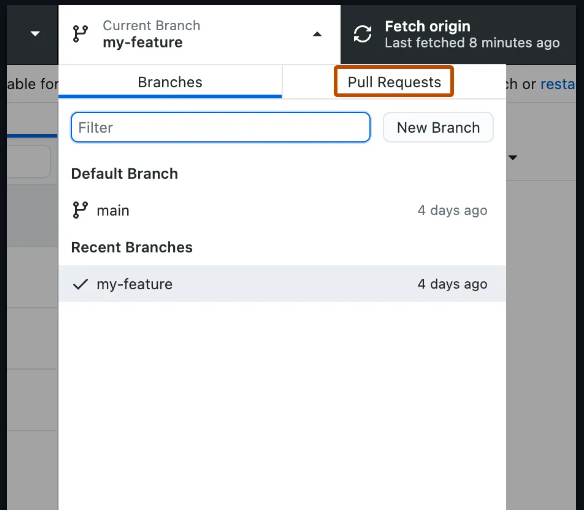
\includegraphics[width=6cm]{images/pull_request.png}
  \end{figure}
  
\end{frame}


\begin{frame}
  \frametitle{Des branches ?}
\ding{81} Créer différentes branches :\\  
  \begin{itemize}
\item \ding{52} peut être utile pour gérer les conflits de version.
\item \ding{52} ça évite à votre collègue d'écraser votre version quand il partage la sienne ou inversement.
\end{itemize}

\ding{81} Mais les branches ça peut être compliqué à gérer. \\
\textcolor{green}{\ding{81}} Au début on peut essayer de travailler sur la même branche : \\
\begin{itemize}
\item \ding{52} Toujours faire un pull avant de push ses propres modifications
\item \textcolor{orange}{\ding{52}} Github prévient en rouge quand il y a un conflit entre la branche locale et la branche serveur !!!
\end{itemize}


\end{frame}

\begin{frame}
  \frametitle{Documentation}

\ding{80} de la documentation, ça peut aider ...\\
\begin{itemize}
\item \ding{229} \url{https://docs.github.com/fr/get-started}
\item \ding{229} \url{https://gist.github.com/Marsgames/2eb2e0321302640efafa4067b483b427}
\end{itemize}


\end{frame}


%\documentclass[xcolor=table]{beamer}

\usetheme{metropolis}
\usepackage{appendixnumberbeamer}
\usepackage[utf8]{inputenc}
\usepackage[russian,francais]{babel}
\usepackage{booktabs}
\usepackage[scale=2]{ccicons}
%\usepackage{xcolor}
\usepackage{wrapfig}
\usepackage{subcaption}
\usepackage{pgfplots}
\usepgfplotslibrary{dateplot}
\usepackage{graphicx}
\usepackage{xspace}
\usepackage{hyperref}
\usepackage{arydshln}
\usepackage{pifont}
\usepackage{enumitem}
\usepackage{xcolor}
\usepackage{minted}
\newcommand{\themename}{\textbf{\textsc{metropolis}}\xspace}
%%\usepackage{polyglossia}
%%    \setdefaultlanguage{french} % main language
%%    \setotherlanguages{russian, hindi, greek, hebrew} % other languages 
%%\graphicspath{{images/}}	% Put all images in this directory. Avoids clutter.
%%\setmainfont{Latin Modern Roman}
%%\setsansfont{Latin Modern Sans}
%%\setmonofont{Latin Modern Mono}
%%\setmainfont[Ligatures=TeX]{Times New Roman}
%%\newfontfamily{\cyrillicfonttt}{Times New Roman}[Script=Cyrillic]

\title{Algorithmique et Programmation (TALA330A L3 INALCO)}
\subtitle{Crédits : Angélique Allaire, ObTIC}
%\subtitle{A modern beamer theme}
\date{17 octobre 2022}
\author{Caroline Koudoro-Parfait\\ \quad {caroline.parfait@sorbonne-universite.fr\\} \quad {}}
\institute{Observatoire des Textes des Idées et des Corpus - Obtic,\\ Sorbonne Center for Artificial Intelligence - SCAI,\\ Sens Textes Informatiques Histoire - STIH EA 4509, Sorbonne Université}
 \titlegraphic{\hfill
\includegraphics[height=.7cm]{images/inalco_logo.png}}




\begin{document}
\maketitle
\definecolor{greenperso}{RGB}{68,117,104}
\definecolor{greenblue}{RGB}{95,179,176}

\begin{frame}{Plan de la présentation}
  \setbeamertemplate{section in toc}[sections numbered]
  \tableofcontents[hideallsubsections]
\end{frame}

\section{Les Fonctions - Principe et généralités}

\begin{frame}{Les Fonctions - Principe et généralités}

\begin{itemize}[label=\textbullet, font= \color{greenperso}]
    \item Utiles pour réaliser plusieurs fois la même opération au sein d'un programme. 
    \item Elles rendent également le code plus lisible et plus clair en le fractionnant en blocs logiques.
\end{itemize}
\end{frame}


\begin{frame}{Les Fonctions natives Python}
    

Vous connaissez déjà certaines fonctions Python. Par exemple des fonctions internes à Python comme :

\begin{itemize}[label=\textbullet, font= \color{greenperso}]
    \item range() : indication pour effectuer une action un certain nombre de fois dans une boucle for
    \item len() : donner la taille d'une liste, d'une chaîne de caractères
    \item print() : affichage
    \item type() : type de la valeur 
\end{itemize}
\end{frame}



\begin{frame}{Les Fonctions}
Pour l'instant, une fonction est à vos yeux une sorte de « boîte noire » (voir figure 1) :
\begin{itemize}[label=\textbullet, font= \color{greenperso}]
    \item À laquelle vous indiquez aucune, une ou plusieurs variable(s) entre parenthèses. Ces variables sont appelées \textbf{arguments}. Il peut s'agir de n'importe quel type d'objet Python.

 \item Qui effectue une action.
\item Et qui renvoie un objet Python ou rien du tout.
\end{itemize}
\end{frame}


\begin{frame}{Les Fonctions}

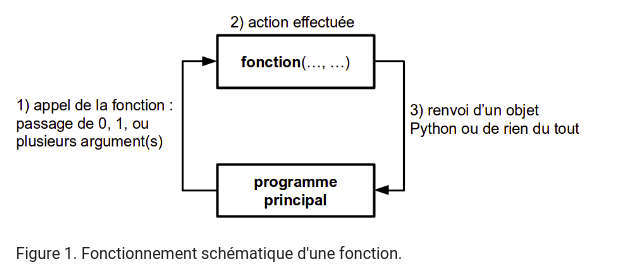
\includegraphics[scale=0.5]{images/fonctions.png}
    
\end{frame}

\section{Déclarer et appeler une fonction}

\begin{frame}{Les Fonctions}

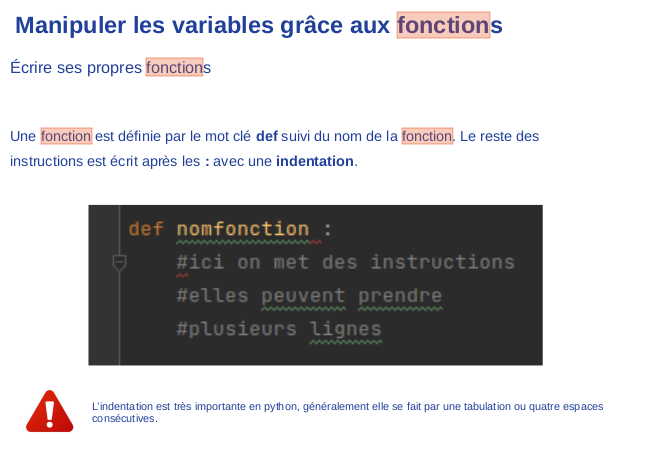
\includegraphics[scale=0.5]{images/fonction_2.png}
    
\end{frame}

\begin{frame}{Les Fonctions}

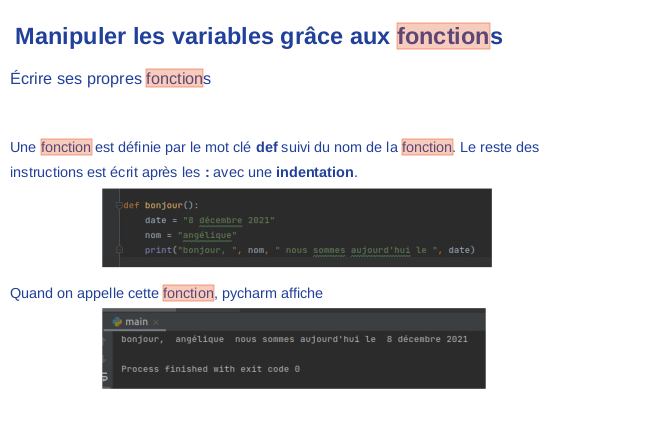
\includegraphics[scale=0.5]{images/fonctions_3.png}
\vspace{-0.3cm}
\footnotesize{$*$ \textit{pycharm} est un IDE, au même titre que \textit{Spyder ou Jupyter notebook}...}
    
\end{frame}

\begin{frame}{Les Fonctions}

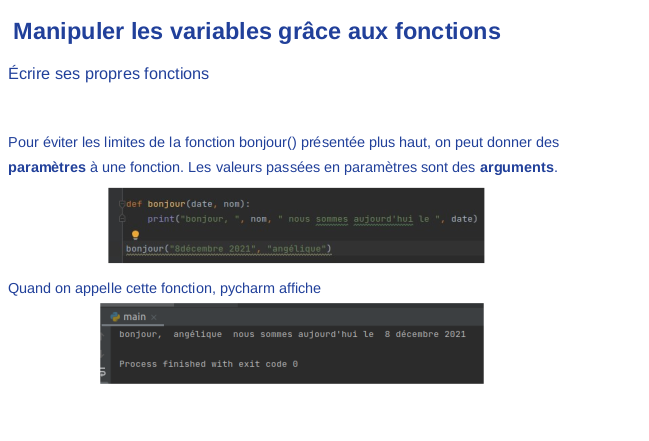
\includegraphics[scale=0.5]{images/fonction_3.png}
\vspace{-0.3cm}
\footnotesize{$*$ \textit{pycharm} est un IDE, au même titre que \textit{Spyder ou Jupyter notebook}...}
    
\end{frame}

\begin{frame}{Les Fonctions}

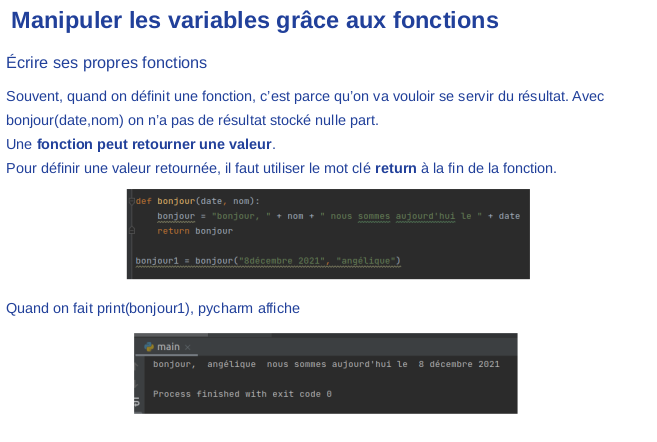
\includegraphics[scale=0.5]{images/fonction-4.png}
    
\end{frame}

\begin{frame}{Les Fonctions}

Exercice :
Écrire une fonction qui retourne l’endroit où nous sommes actuellement et ce que nous faisons en utilisant des paramètres
    
\end{frame}


\begin{frame}{Les Fonctions}
Ecrire la fonction 
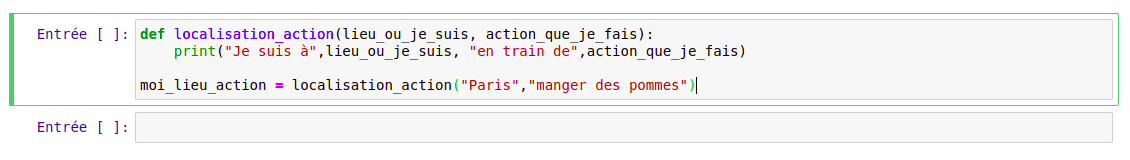
\includegraphics[scale=0.3]{images/fonction_1.png}
\pause

\vspace{1cm}
Quand on fait tourner le programme on obtient : 
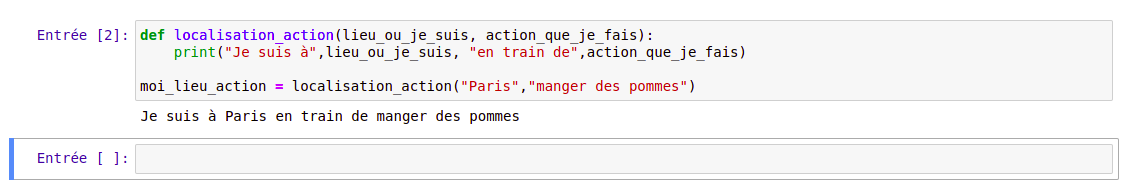
\includegraphics[scale=0.3]{images/fonction2.png}

\end{frame}
\end{document}

%\begin{frame}[allowframebreaks]
%        \frametitle{References}
%%\bibliographystyle{apalike}
%%\scriptsize{
%%\bibliography{biblioCM2}}
%\end{frame}

\end{document}
